\chapter{Diseño de la solución}
\par Como es habitual en los Proyectos de Fin de Grado, uno de los retos más interesantes que se encuentran consiste en afrontar, abrazar y controlar la
incertidumbre sobre cómo será la solución final; dicha incertidumbre es inherente a todo proyecto de software, pero en un PFG es mayor debido a que la
investigación tiene a su vez un mayor peso y es determinante.
\par En el presente proyecto, a la hora de afrontar inicialmente el diseño de la solución se desconoce qué tecnologías se van a utilizar específicamente y éstas
se deciden tras evaluarlas tanto individualmente como su capacidad de integración entre ellas y con elementos externos.
\par Para ello se sigue un modelo de desarrollo evolutivo similar al modelo de prototipos. Para lo cual se parte de la definición de un diseño a alto nivel en
el que se definen los componentes y sus funciones más representativas. A continuación se empieza a realizar un proceso iterativo en el que se van probando los
componentes y añadiendo nuevos elementos. El resultado de dicha fase es una solución funcional inicial que cumpla los requisitos definidos. Sobre dicho modelo
se realiza una revisión de calidad que permita contar con una solución suficientemente madura y estable.
\par No obstante, dado que se espera que la solución sea algo en constante cambio, se ha elegido una metodología de desarrollo ágil~\cite{wiki:agil}, tal como
se describe más adelante.

\section{Componentes principales}
\par Estos son los componentes que se han identificado para la solución:
\begin{itemize}
  \item El primer componente que se ha identificado es un WAF con licencia de software libre. Este elemento es el componente más importante de la solución y
    marca en gran medida los demás componentes que participen en la capa de aplicación.
    \par Durante la fase de construcción se evalúan qué componentes WAF cumplen los requisitos y se elige un candidato.
  \item El segundo componente de la solución es el software responsable de gestionar las comunicaciones HTTPS. Este software es el encargado de cifrar y
    descifrar el tráfico SSL / TLS.
  \item El tercer componente es el software de virtualización o de contenedores. Uno de los puntos clave de la solución es garantizar la facilidad para
    implementarla de forma poco intrusiva. Para ello se considera que un software de contenedores como Docker~\cite{docker}. Este tipo de soluciones está
    ampliamente asentada en el mercado y existe un movimiento significativo de migración de los entornos tradicionales a entornos de contenedores.
  \item Otro componente estrechamente relacionado con el componente anterior es el software automatización de despliegue y gestión de la solución. Este
    componente es opcional y por lo tanto se tendrá en cuenta que la opción deber ser sustituible en diferentes implementaciones con el fin de garantizar la
    máxima portabilidad de la solución.
  \item Otro componente del que depende la solución es el conector con los elementos de almacenamiento persistente. Este componente es el encargado de
    proporcional un servicio de compartir información entre recursos y garantizar la perdurabilidad de la información necesaria. Se hará foco en reducir el uso
    o impacto de este componente al mínimo y que todo el entorno pueda ser reconstruido con el menor esfuerzo posible con el fin de ofrecer un entorno dinámico
    siguiendo los principios \acrshort{cicd} ya mencionados.
  \item Por último, tenemos dos componentes directamente relacionados con la personalización de la herramienta por el usuario final. Se trata de las reglas de
    auditoría o bloqueo del WAF, así como las reglas de configuración del software de TLS. Estos componentes serán los ficheros o parámetros de configuración de
    los dos primeros componentes que se han identificado.
\end{itemize}

\section{Construcción de la solución}

\par Tal como se comentaba anteriormente, debido al alto grado de incertidumbre que se tiene del aspecto final de la solución, junto con la necesidad de poder
realizar cambios sobre el modelo de forma rápida, se ha optado por seguir una metodología de desarrollo ágil~\cite{wiki:agil}.
\par Durante el proceso de desarrollo del proyecto se utilizará como referencia o mantra el \Gls{ManifiestoAgil} y como modelo de liberación de versiones se
siguen los principios de integración continua, entrega continua (en adelante \acrshort{cicd}, de sus siglas en inglés, \acrlong{cicd}).

\section{Análisis y selección de tecnologías}
\par En esta sección se evalúan las distintas opciones disponibles y se elige una tecnología candidata sobre la que construir la solución.
\subsection{Web Application Firewall}
\par En primer lugar, de acuerdo a los requerimientos establecidos - {~\hyperref[req:softwarelibre]{La plataforma debe ser compatible con el modelo de
licencias de software libre}} - se han descartado las soluciones WAF privativas y aquellas que no estén licenciadas bajo una licencia del tipo GPL.  En
este segundo grupo se encuentran WebKnight - sólo compatible con el software de aplicación web Internet Information Services\cite{iis} sobre plataformas
Microsoft Windows - y Vulture, con licenciamiento BSD y que requiere un sistema operativo FreeBSD.

\par Otras soluciones se han descartado debido a que están discontinuadas desde hace tiempo, como IronBee que no se ha actualizado desde hace más de 3 años
y WebCastellum desde hace 5 años.

\par Otra tecnología candidata que se ha descartado ha sido RAPTOR debido a que no soporta tráfico SSL/TLS ({~\hyperref[req:tls]{La solución debe poder
participar en la negociación TLS}}).

\par NAXSI se ha considerado que no cumple los requisitos básicos que debe tener un WAF actualmente ({~\hyperref[req:commonattacks]{La solución debe
disponer de un conjunto básico de políticas de auditoría o bloqueo que permitan proteger la aplicación web frente a los ataques más comunes}}), pues
sólo implementa dos controles de seguridad - de los referenciados en el documento de buenas prácticas de OWASP\cite[apartado A3.2]{owaspbestpractices});
concretamente, sólo protege ataques de tipo {\em Cross-site scripting} (en adelante \acrshort{xss}\cite{owaspxss}) e inyecciones SQL (en adelante
\acrshort{sqli}\cite{owaspsqli}). Además, se han producido duras críticas acerca de las funcionalidades que ofrece \cite{naxsianalisis}.

\par OpenWAF por su parte es una iniciativa con un planteamiento y unas funcionalidades muy interesantes, pero que lleva más de dos años sin
publicar una nueva versión y además carece de suficiente madurez para considerarse su uso en un entorno de producción (la última versión
publicada es la 0.0.4).

\par Respecto a FreeWAF (también conocido como {\em lua-resty-waf}) está en una situación muy similar a OpenWAF, pues su última versión tiene más de 2
años y se trata de la versión 0.11.1\cite{freewafchangelog}.

\par En el caso de Shadow Daemon, no se cumple el requisito de independencia ({~\hyperref[req:independence]{La solución debe poder ejecutarse en un
sistema operativo o máquina independiente de la plataforma de la aplicación web}}), pues se trata de un conector de aplicación web con una
funcionalidades interesantes, pero por diseño requiere de su integración con el framework de desarrollo y sólo es compatible con PHP, Perl y Python. Por
lo tanto no es posible implementarlo como elemento externo e independiente de la plataforma web.

\par Por último, se ha considerado ModSecurity. Esta tecnología está disponible en dos ramas de desarrollo, la rama 2.x (versión 2.9.3 en el momento en
el que se escribe este documento) y la rama 3.x (versión 3.0.3 actualmente).
\par La rama no cumple los requisitos de independencia ({~\hyperref[req:independence]{La solución debe poder ejecutarse en un sistema operativo o
máquina independiente de la plataforma de la aplicación web}}), debido a que se despliega como un módulo de Apache y no permite que su despliegue sea
agnóstico de la plataforma web; por lo tanto se descarta esta versión de ModSecurity.

\par La rama 3.x por el contrario incorpora entre sus novedades una reescritura completa del código y la posibilidad de enlazarse a distintas
tecnologías de servicios web.

\par Cabe mencionar que las tecnologías que abiertamente no cumplen los requisitos definidos se han descartado, pero aquellas que cumplen con los
requisitos pero que llevan tiempo sin actualizarse o están en una fase temprana de desarrollo se mantienen como opciones alternativas en caso de que la
opción candidata no cumpla con las expectativas.
\subsubsection{Tecnología candidata}
\par Se ha elegido como tecnología candidata ModSecurity en su versión 3.x, pues cumple todos los requisitos y es un referente entre las tecnologías de
WAF de software libre.

\subsection{Servicio web}
\par Uno de los componentes sobre los que se debe apoyar el WAF es el servicio web. Este componente se comporta como un interfaz entre el WAF y las peticiones y respuestas del cliente y el servicio web.
\par Se han identificado los siguientes servicios web compatibles con  ModSecurity en su versión 3:
\begin{itemize}
  \item Internet Information Services (IIS)~\cite{iis}.
  \item Apache HTTP Server (Apache)~\cite{apache}.
  \item Nginx~\cite{nginx}.
\end{itemize}
\par IIS se ha descartado debido a que sólo es compatible con plataformas Windows, tal como se comentó en la sección ~\nameref{subsec:estadoarte}.

\par Tanto Apache como Nginx cumplen los requisitos funcionales, pero Nginx tiene mejores capacidades de proxy inverso.

\par Respecto al licenciamiento, Nginx utiliza {\em Licencia BSD simplificada o licencia FreeBSD (de 2 cláusulas)}~\cite{wiki:SimplifiedBSDLicense}, la cual es compatible con GPL.

\subsubsection{Tecnología candidata}
\par Se ha elegido como servicio web Nginx.

\subsection{Software criptográfico}
\par Uno de los puntos clave para proporcionar un canal cifrado y seguro alineado con las mencionadas mejores prácticas de TLS ~\cite{TLSBestPractices} o de PCI DSS~\cite{pcidssrequirements} es el uso de TLS en su versión 1.3 y HTTP/2.
\par Se han descartado por lo tanto las soluciones que no cumplen estos requisitos, como por ejemplo LibreSSL~\cite{libressl}.
\par Una vez realizado este primer filtro, se han seleccionado las siguientes opciones:
\begin{itemize}
  \item GnuTLS~\cite{gnutls}.
  \item OpenSSL~\cite{openssl}.
  \item Network Security Services (NSS~\cite{nss}).
\end{itemize}

\par A la hora de valorar estas opciones se ha identificado que a nivel de licenciamiento, sólo GnuTLS utiliza una licencia de tipo GPL.
\par Sin embargo, uno de los componentes previamente seleccionados - Nginx - sólo es compatible con OpenSSL~\cite{opensslnginx}.
\par OpenSSL por su parte tiene una licencia doble, licencia ~\cite[Apache License 1.0]{apachelicense10} y \cite[licencia SSLeay]{ssleaylicense}, esta última heredada del proyecto original en el que se basa OpenSSL.

\par Para resolver este problema se han identificado diferentes opciones:
\begin{enumerate}
  \item Cambiar Nginx por una alternativa que soporte GnuTLS.
  \item Desplegar los componentes de cifrado y de WAF en sistemas independientes.
  \item Revisar la compatibilidad de licencias.
\end{enumerate}

\par Para evaluar la viabilidad de la primera opción se han identificado qué servicios son compatibles con GnuTLS. Según la Wikipedia~\cite{wiki:gnutls} este proyecto es usado principalmente en clientes TLS y sólo es compatible con el servicio
web Apache, el cual a su vez tiene el mismo tipo de licencia que OpenSSL (Apache License). Por lo que tiene la misma incompatibilidad de licencias ya mencionada.

\par Debido a la falta de compatibilidad de GnuTLS con otros servicios web, la segunda opción mantiene la dependencia de Apache y su licencia, por lo que  se debe descartar igualmente esta opción.

\par Para evaluar la tercera opción, dado que la librería OpenSSL es una de las más utilizadas, se ha investigado cual es el acercamiento que otros proyectos de software libre.
\par El acercamiento de algunos proyectos es utilizar una licencia tipo GPL modificada en la que se añade una excepción para esta librería~\cite{opensslexception}. Esta solución la han seguido proyectos como {\em GNU Wget} y {\em climm}. Para
ello se deben adjuntar archivos binarios dentro del proyecto y modificar la licencia GPL ofrecida por la GNU; si bien es una opción viable, no es la opción deseable.
\par Investigando cual es el acercamiento de otros proyectos para mantener su licencia GPL y utilizar OpenSSL, se ha identificado que OpenSSL ha iniciado un proceso de cambio de licencia para atajar este problema. Para ello han decidido
cambiar su licencia por una compatible con GPL (~\cite[Anuncio del cambio de licencia]{opensslannouncement}). El cambio de licencia se ha aplicado recientemente (\cite[{\em Pull request} del cambio]{opensslpullrequest}) y ya es efectivo en las
versiones proporcionadas por la versión {\em Buster} de Debian GNU/Linux.
\par Con este cambio se elimina la incompatibilidad de licencias que se había identificado.

\subsubsection{Tecnología candidata}
\par Se ha elegido como tecnología candidata OpenSSL, pues cumple todos los requisitos y es una de las librerías más extendidas y probadas.

\subsection{Software de virtualización}
\par A la hora de elegir software de virtualización, todas las soluciones que se conocen cumplen con los requisitos y objetivos del proyecto, por lo que se ha optado por Docker debido a que es una solución ampliamente utilizada y en constante
expansión.

\subsubsection{Tecnología candidata}
\par La solución que se ha elegido es \cite{docker}.

\subsection{Software de automatización u orquestación}
\par Esta tecnología será la responsable de garantizar el cumplimiento de los siguientes requisitos:
{~\hyperref[req:facilidad]{La plataforma debe ser fácilmente integrable en la plataforma web del cliente.}}
{~\hyperref[req:escalado]{Escalabilidad. La plataforma debe permitir la ampliación o reducción de recursos de forma dinámica.}}

\par Para poder ofrecer estas funcionalidades, se han evaluado las siguientes tecnologías:
\begin{itemize}
  \item Kubernetes (K8s)~\cite{kubernetes}.
  \item Apache Mesos~\cite{mesos}.
  \item Docker Swarm~\cite{swarm}.
\end{itemize}

\par Todas las tecnologías cumplen las necesidades funcionales definidas y todas ellas tiene un licenciamiento compatible con las licencias de tipo GPL.

\par Para poder ofrecer que la solución sea fácilmente integrable, se ha evaluado el uso de estas soluciones y se ha comprobado como Kubernetes es la solución más ampliamente extendida (ver los gráficos
{~\hyperref[fig:KubernetesSwarm]{Kubernetes y Docker Swarm}} y {~\hyperref[fig:KubernetesMesos]{Kubernetes y Apache Mesos}}).

\begin{figure}[hp]
  \centering
  \label{fig:KubernetesSwarm}
  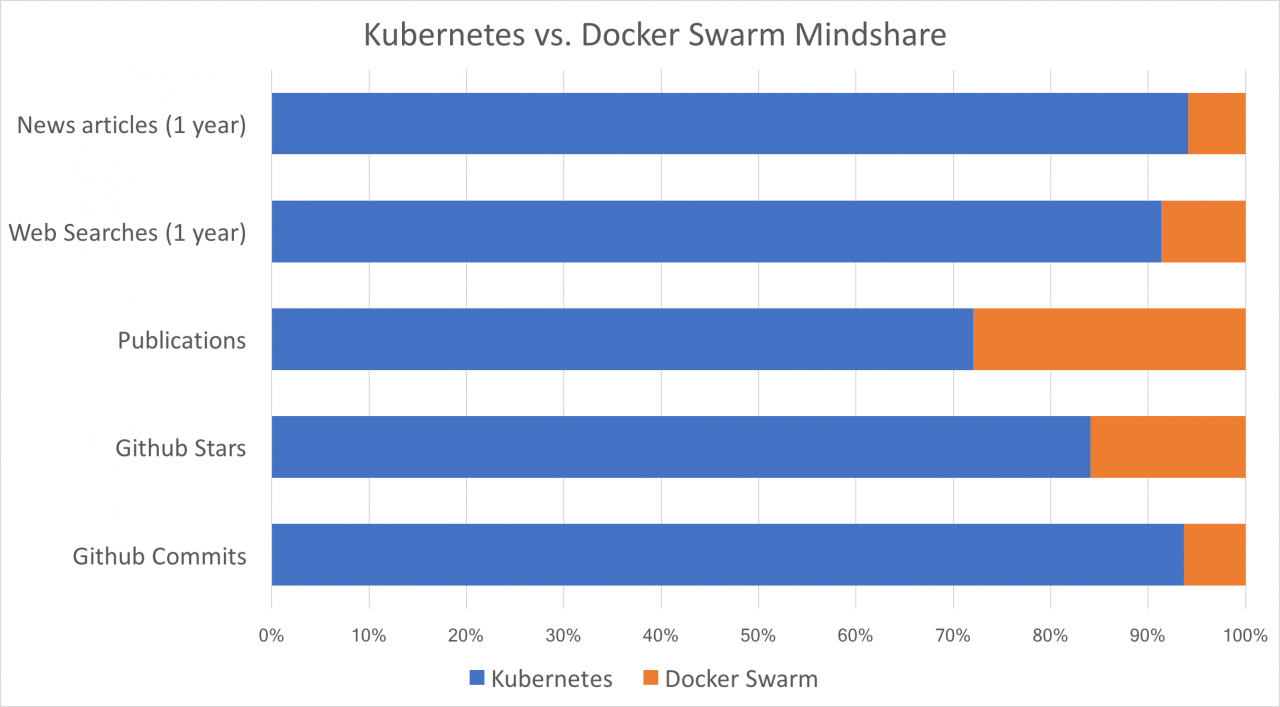
\includegraphics[width=0.7\textwidth]{fig/KubernetesSwarm}
  \caption{Uso y popularidad de software de Kubernetes y Docker Swarm(fuente Platform9~\cite{KubernetesSwarm})}
\end{figure}

\begin{figure}[hp]
  \centering
  \label{fig:KubernetesMesos}
  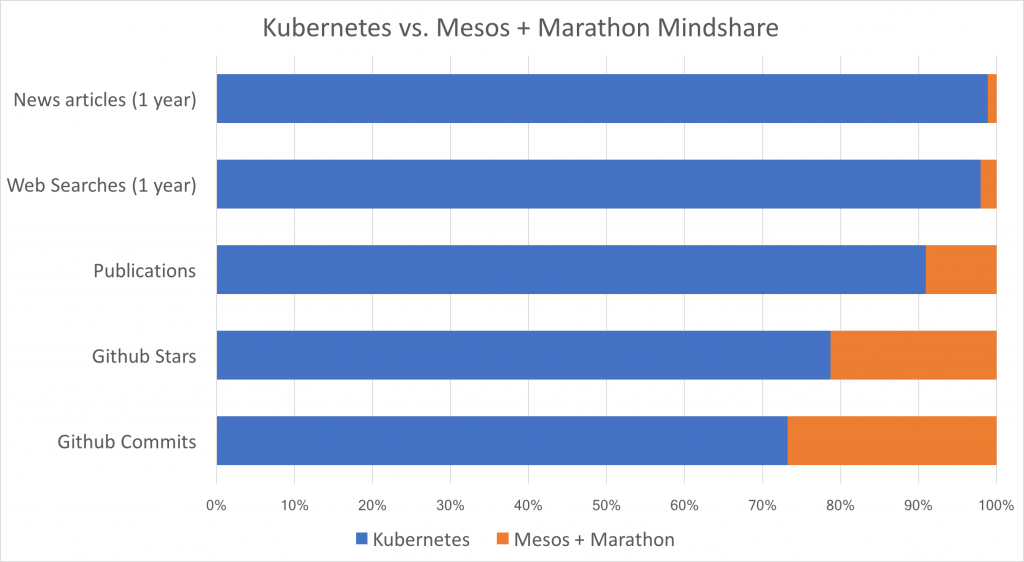
\includegraphics[width=0.7\textwidth]{fig/KubernetesMesos}
  \caption{Uso y popularidad de software de Kubernetes y Apache Mesos(fuente Platform9~\cite{KubernetesMesos})}
\end{figure}

\par Si además comparamos la evolución que estas tecnologías han tenido históricamente, la diferencia es aun mayor como se puede comprobar en el gráfico de {~\hyperref[fig:orquestatorspopularity]{Popularidad de software de orquestación}}. 
\begin{figure}[hp]
  \centering
  \label{fig:orquestatorspopularity}
  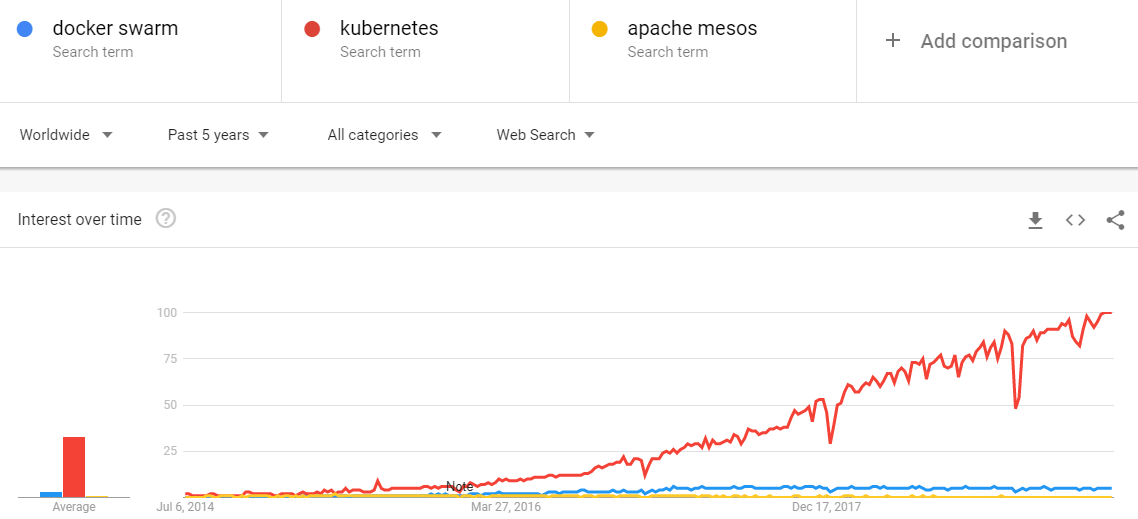
\includegraphics[width=0.7\textwidth]{fig/KubernetesSwarmMesos}
  \caption{Histórico de popularidad de software de orquestación (fuente Google~\cite{KubernetesSwarmMesos})}
\end{figure}

\par Cabe mencionar que existen soluciones Kubernetes adaptadas a los entornos de los principales proveedores del Cloud, como son {\em Azure Kubernetes Service (AKS)~\cite{aks}} o
{\em Amazon Elastic Kubernetes Service (Amazon EKS)~\cite{eks}}. Estas soluciones cuentan con la ventaja de que facilitan su despliegue y mantenimiento mediante
el uso de herramientas propias, pero cuentan con una fuerte desventaja: Aumentan la cautividad de la solución con un único proveedor.
\par Sin embargo, la migración de una solución agnóstica del proveedor del Cloud a un proveedor específico es sencilla.
\par Por lo tanto se ha optado por no utilizar ninguna solución específica del Cloud y utilizar la tecnología Kubernetes sin funcionalidades añadidas como son
los {\em Ingress Controllers~\cite{ingresscontrollers}} o API de proveedores del Cloud. Esto permitirá que la solución sea fácilmente desplegable en el mayor
número de entornos posible.

\subsubsection{Tecnología candidata}
\par Se ha elegido Kubernetes~\cite{kubernetes} como tecnología candidata para implementar la automatización de la plataforma.

\subsection{Servicio de almacenamiento}
\par El objetivo de este componente es garantizar un servicio de intercambio de información entre los distintos componentes de la misma y, en caso de que sea
necesario, el almacenamiento persistente de la información. Pero, tal como se ha comentado anteriormente, se intentará minimizar su uso. De ser posible se
utilizará alguna solución ya presente en la infraestructura.
\par Entre las soluciones a evaluar existen dos aproximaciones posibles: Servicios tradiciones como Samba ~\cite{samba} o  NFS (estándar RFC7530~\cite{nfs}) o
servicios del Cloud como Amazon S3\cite{s3} o Google Storage\cite{GoogleStorage}.

\par Tal como se ha identificado a la hora de identificar la tecnología de automatización, las soluciones proporcionadas por los fabricantes del Cloud limitan
las posibles plataformas que adopten la solución, por lo que se prefiere utilizar servicios de almacenamiento e intercambio de archivos independientes del
proveedor.
\par Tanto Samba como NFS cubren los requisitos, por lo que cualquiera de estas tecnologías son válidas. Sin embargo, dentro de los entornos de contenedores el
protocolo NFS está más extendido.

\subsubsection{Tecnología candidata}
\par Se utilizará por tanto un servicio de almacenamiento basado en ~\cite{nfs}, preferiblemente un recurso externo a la solución propuesta.

\subsection{Políticas o reglas de auditoría}

\subsubsection{Tecnología candidata}


